%%%%%%%%%%%%%%%%%%%%%%%%%%%%%%%%%%%%%%%%%%%%%%%%%%%%%%%%%%%%%%%%%%%%%%%%%%%%%%%%
%2345678901234567890123456789012345678901234567890123456789012345678901234567890
%        1         2         3         4         5         6         7         8

\documentclass[letterpaper, 10 pt, conference]{ieeeconf}  % Comment this line out
                                                          % if you need a4paper
%\documentclass[a4paper, 10pt, conference]{ieeeconf}      % Use this line for a4
                                                          % paper
\usepackage{graphicx}
\usepackage{amsmath}
\usepackage{graphicx}
\usepackage{subcaption}

\IEEEoverridecommandlockouts                              % This command is only
                                                          % needed if you want to
                                                          % use the \thanks command
\overrideIEEEmargins
% See the \addtolength command later in the file to balance the column lengths
% on the last page of the document

% The following packages can be found on http:\\www.ctan.org
%\usepackage{graphics} % for pdf, bitmapped graphics files
%\usepackage{epsfig} % for postscript graphics files
%\usepackage{mathptmx} % assumes new font selection scheme installed
%\usepackage{times} % assumes new font selection scheme installed
%\usepackage{amsmath} % assumes amsmath package installed
%\usepackage{amssymb}  % assumes amsmath package installed

\title{\LARGE \bf
Multimedia Feature Generation of Movie Trailers for Genre Prediction\\
}

\author{Nathaniel Guy, John Fuini and Yong Han Noel Kim\\
	University of Washington, Seattle WA% <-this % stops a space
\thanks{Nathaniel Guy and Yong Han Noel Kim are Masters students in the University of Washington Department of Aeronautical and Astronautical Engineering, and can be reached at {\tt\small natguy@cs.washington.edu} and {\tt\small kimber.noel@outlook.com}, respectively. John Fuini is a PhD student in the University of Washington Department of Physics, and can be reached at {\tt\small fuini@uw.edu}. }%
}
\date{ \today}

\begin{document}

\maketitle
\thispagestyle{empty}
\pagestyle{empty}

%%%%%%%%%%%%%%%%%%%%%%%%%%%%%%%%%%%%%%%%%%%%%%%%%%%%%%%%%%%%%%%%%%%%%%%%%%%%%%%%
\begin{abstract}



\end{abstract}

%%%%%%%%%%%%%%%%%%%%%%%%%%%%%%%%%%%%%%%%%%%%%%%%%%%%%%%%%%%%%%%%%%%%%%%%%%%%%%%%
\section{INTRODUCTION}
Movie trailers are one of the most effective advertising tools for the film industry. They deliver relevant information such as background, cast, theme, plot and more, in a limited amount of time. As such, trailers can be considered a subset of a movie which contains its principal components. With this idea in mind, we developed an algorithm which classifies movie trailers by their genre. This is a familiar process to all movie-viewers: movie viewers are generally able to tell if a certain movie is a comedy film, action film, documentary, etc. within the first minute of watching a trailer based on myriad cinematic features within it. Viewers have developed this cognitive ability by watching countless movies of various genres over time, and have subconsciously learned to identify the cinematic features associated with certain genres. Our algorithm is an adaptation of this process using machine learning. This report describes our process of identifying cinematic features from a large set of trailers of known genre, training a machine learning algorithm to develop classification criteria based on these features and genre metadata, and testing the generated classification criteria on a set of trailers to assess the effectiveness of our approach.

%%%%%%%%%%%%%%%%%%%%%%%%%%%%%%%%%%%%%%%%%%%%%%%%%%%%%%%%%%%%%%%%%%%%%%%%%%%%%%%%
\section{RELATED WORK}
Zeeshan Rasheed et al. in their \textit{On the Use of Computable Features for Film Classification}\cite{Rasheed}, developed an algorithm for film classification based on film previews. They limited themselves to visual features only, such as average shot length, color variance, motion content and lighting key, and four genres: comedy, action, drama and horror. We aimed to create a more robust algorithm that can classify 25 genres, using more features from both visual and audible features.


%%%%%%%%%%%%%%%%%%%%%%%%%%%%%%%%%%%%%%%%%%%%%%%%%%%%%%%%%%%%%%%%%%%%%%%%%%%%%%%%
\section{COMPONENT ARCHITECTURE}
\subsection{Feature Generation via Video Processing}
%keyword : regex, OpenCV2, 
The majority of video processing was done using open source Python module, OpenCV2. 
\subsubsection{Number of Frames}
CV2 can measure the frame per second (FPS) for a given trailer. A feature 'number of frames' was calculated by dividing the total run-time of a trailer by its FPS.
\subsubsection{Total Time}
Total time feature is a total run-time of a trailer.
\subsubsection{Average Intensity}
Average greyscale intensity was calculated using standard weights:
\begin{equation*}
Average\,intensity= 0.2989R+0.5870G+0.1140B
\end{equation*}
\subsubsection{R, G and B Component}
R, G and B components denote the proportion of R, G and B colors for a given frame. Average values of these in a trailer was calculated. A certain portion of the trailer was a letterbox, and could be dropped from the average judging by the fact that pixels pertaining to the letterbox have all zero values for color. Nonetheless, the size of letterbox varied from a trailer to a trailer, and writing a modular code that calculates the standard deviation of colors excluding the letterbox was challenging. Thus the standard deviation of R, G, and B color components were calculated with letterboxes.

\subsubsection{Number of Shots}
We detected a shot transition by examining color histograms of each frames. When the chi-squared distance between two histograms exceed the shot transition threshold, we assumed there was a transition of shot between two frames. One disadvantage to this method is that algorithm cannot differentiate between fast camera moves and complete change of shots, as with fast camera moves, the color histogram from frame-to-frame varied as rapidly as actual shot transition.
\subsubsection{Shot Length}
%mean, std dev,min and max
Once the time-stamps of shot transitions were recognized, we were able to calculate mean, standard deviation, minimum and maximum shot lengths. The mean shot length varied greatly from 0.2 s. to 3 s.
\subsubsection{Detail Score}
%std dev, min and max
We defined detail score as a measure of visibility of edges and other fine details present in a trailer. An edge detection algorithm analyzed each individual frame in a trailer, and provided statistics such as mean value, standard deviation, minimum and maximum values of detail score.
\subsubsection{Dark Scene}
%count, percentage, mean length, std dev, min and max
Dark scene was defined as a period of time when dark frames persisted. Their lengths were recorded, from which mean length, standard deviation of length, minimum and maximum lengths were calculated. The percentage of dark scenes in the entirety of the trailers was also calculated. 

\subsection{Feature Generation via Audio Processing}
%kewword : FFT, 
From the trailers saved in video file format, we extracted the audio component using sampling frequency of 44.1 kHz. A series of analysis was done on this audio component to extract features.
\subsubsection{Volume}
\textit{Mean} : Mean volume for each trailer was calculated by averaging the amplitudes of sound waves over the entire duration of a trailer. A motivation behind extracting this feature was that a trailer saturated with loud noises would have bigger value of mean volume than movies with relatively calm sound. And naturally, trailers with loud noises - explosion, jet noise, shouting, etc. are associated with genres such as action, thriller, adventure. On the other hand, trailers with calm audio, and even some quietness could be associated with genres such as drama, history, family. \\
\textit{Standard Deviation}: While all trailers were sourced from a single source, there was no guarantee that they were equalized to the same degree. Thus, a higher mean volume could simply mean a sheer loudness of overall volume. In order to get a sense of how much variation of volume is in each trailer, we calculated standard deviation of the sound waves over the entire trailer as well.\\
\textit{Minimum and Maximum}: Minimum and maximum volume for each trailer were calculated based on the waveform. Most trailers had minimum volume near zero, while some had marginally higher value such as 0.03. For a perspective, maximum volume ranged from values of 0.1 to 0.5, roughly.
\subsubsection{Sudden Rise/Fall of Volume}
The sudden rise and sudden fall of volume were defined as an increase and a decrease of volume with a magnitude bigger than the standard deviation of volumes, respectively. 
\subsubsection{Percentage of Sound Corresponding to Different Octave Bands}
For this feature, the waveform of each trailer was transformed to the frequency domain using Fast Fourier transform (FFT). Its frequencies were divided into eleven bands commonly defined as octave band (11Hz \sim 22720Hz). The magnitudes of frequency components in each band were summed together, and normalized so that the sum of magnitudes of all octave bands would be 1. The resulting magnitudes represented the composition of sounds of each trailer with respect to eleven octave bands. 

\subsection{Use of Features in Machine Learning Algorithm}
%keyword: binary decision tree
All extracted features from each movies were compiled into a single *.CSV spreadsheet. In addition to features, the spreadsheet contained the genre labels of each movies as well. Movies were not limited to one genre. For instance, there were movie trailers with multiple genre labels such as action-comedy, or mystery-horror-thriller. This spreadsheet was passed on to Matlab's fit binary classification decision tree function (\textit{fitctree}) to build a decision tree. Only 80\% of the trailers randomly selected from the full set of trailers were used for building the tree. This subset is known as a trainer set. The tree was then used to predict the entire range of trailers using Matlab's classification predict function (\text{predict}), and its success and failure rate were recorded. This process was repeated 40 times, each time with a new set of random trainer sets, for the purpose of cross-validation. 



%%%%%%%%%%%%%%%%%%%%%%%%%%%%%%%%%%%%%%%%%%%%%%%%%%%%%%%%%%%%%%%%%%%%%%%%%%%%%%%%
\section{RESULTS}
The rate of successive classification by our algorithm for top ten most popular genres are shown in fig. \ref{f:success_rate_table}. The Drama, with 65\% successful classification, had the lowest success rate of them, but the rest registered consistently over 80\% success rate.\\
\begin{figure}[h]
	\centering
	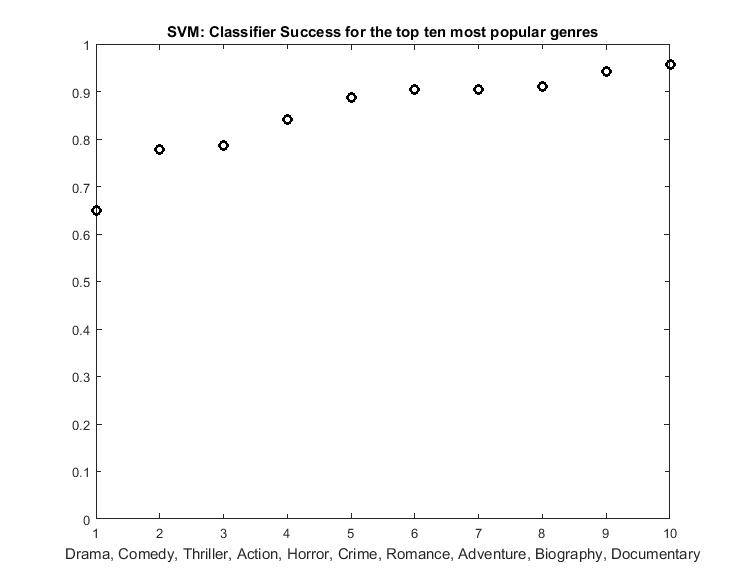
\includegraphics[width=\columnwidth]{success_rate.jpg}
	\caption{Classifier success rate for ten most popular genres.}
	\label{f:success_rate_table}
\end{figure}
In order to gain some insight to what features are important for the classification, we performed singular value decomposition on the set of movie trailers and their features. As can be seen in the plot of covariances of principal modes (fig. \ref{f:mode_covar}), only four modes capture roughly 90\% of the energy.
\begin{figure}[h]
	\centering
	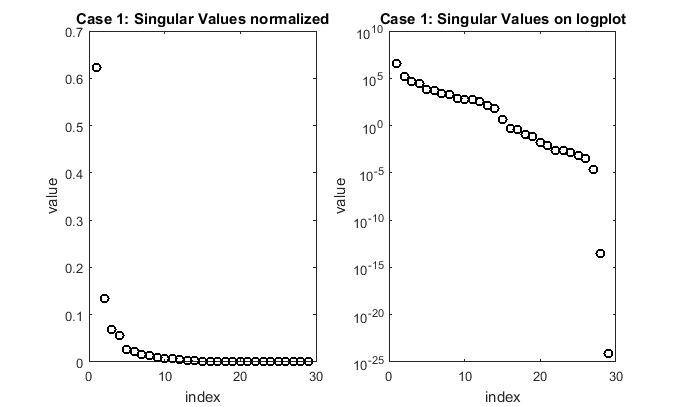
\includegraphics[width=\columnwidth]{mode_covar.jpg}
	\caption{Covariances of modes}
	\label{f:mode_covar}
\end{figure}
These four modes consist of features of differing degree. Figure \ref{f:mode_composition} display the weights of each feature in four prominent modes. One can observe that the leftmost ten features are driving factors for these modes. These features are: number of shots, dark scene max. length, total time, average blue color, average green color, average intensity, average red color, dark scene length standard deviation, dark scene mean length and dark scene count. This results suggest that machine learning algorithm relies mainly on chromatic and luminous qualities of trailers, as eight out of ten most important features describe color and brightness of scenes in trailers. In another words, from a machine's perspective, trailers of different genres sound similar, but some are more colorful than the other.
\begin{figure}[h]
	\centering
	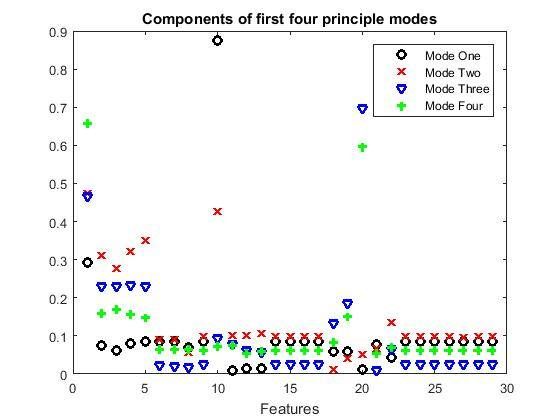
\includegraphics[width=\columnwidth]{mode_comp.jpg}
	\caption{Compositions of features for each modes}
	\label{f:mode_covar}
\end{figure}
We experimented with the concept of dimension reduction by trying the classification using one, two and four modes. The rate of success are plotted in fig. \ref{f:modal_redx}. Surprisingly, the difference of success rate between one-mode classification and all-mode classifications are only about 10\%.
\onecolumn
\begin{figure}
	\centering
	\begin{subfigure}[b]{0.475\textwidth}
		\centering
		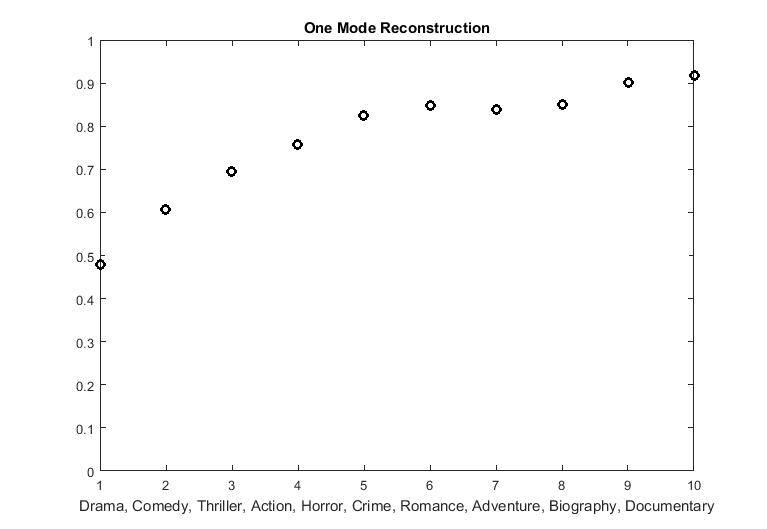
\includegraphics[width=\textwidth]{one_mode_appx}
	\end{subfigure}
	\hfill
	\begin{subfigure}[b]{0.475\textwidth}  
		\centering 
		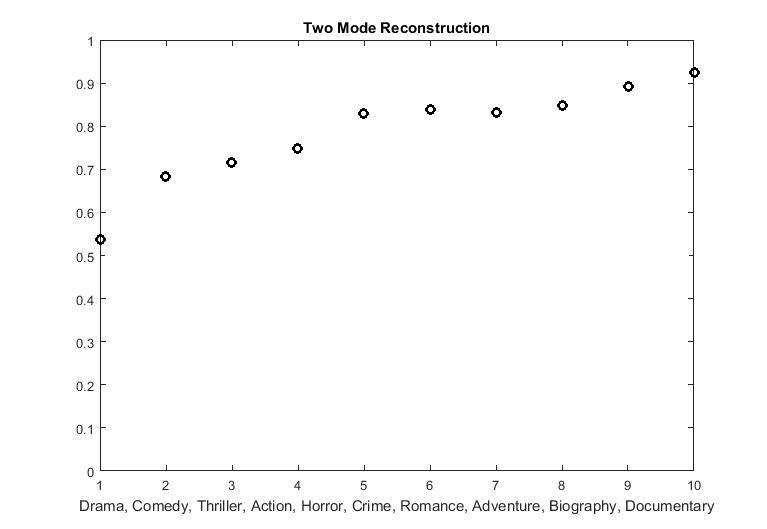
\includegraphics[width=\textwidth]{two_mode_appx}
	\end{subfigure}
	\vskip\baselineskip
	\begin{subfigure}[b]{0.475\textwidth}   
		\centering 
		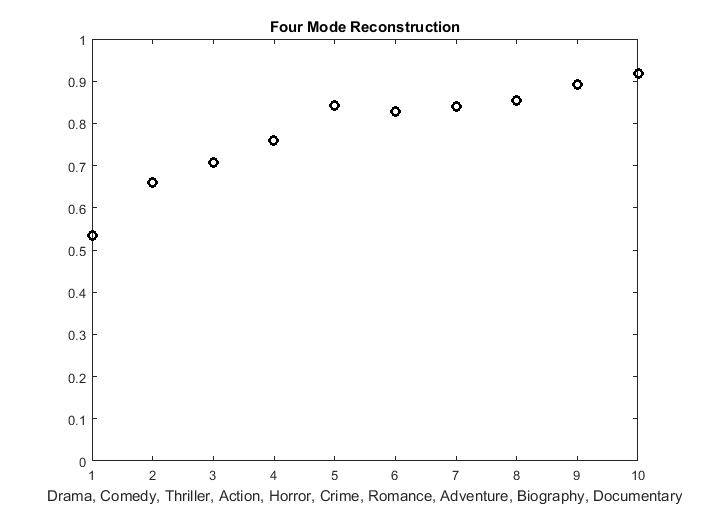
\includegraphics[width=\textwidth]{four_mode_appx}
	\end{subfigure}
	\quad
	\begin{subfigure}[b]{0.475\textwidth}   
		\centering 
		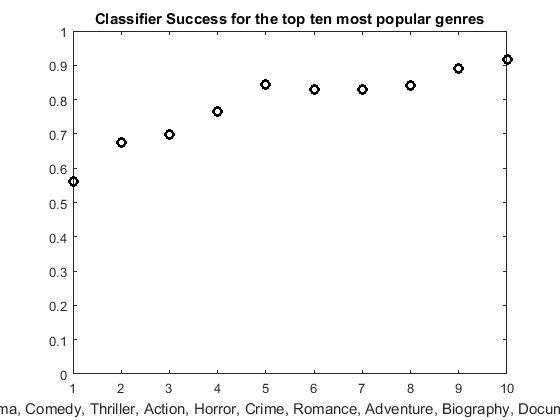
\includegraphics[width=\textwidth]{orig_mode}
	\end{subfigure}
	\caption{Classifications made with one, two and four mode approximation compared to the original classification made with a complete set of modes} 
	\label{f:modal_redx}
\end{figure}

\twocolumn

%%%%%%%%%%%%%%%%%%%%%%%%%%%%%%%%%%%%%%%%%%%%%%%%%%%%%%%%%%%%%%%%%%%%%%%%%%%%%%%%
\section{LESSONS LEARNT}
One failed attempt to acquire features from the audio portion of movie trailers was to perform a principal component analysis using singular value decomposition. The goal of this process was to identify a series of principal modes and their components in each movie trailers. The values of principal components could be used as features. We clipped  10-second portion of audio from each trailer to reduce the size of the data. Nonetheless, the matrix at which the singular value decomposition was to be performed had a size of 958-by-227150. This was computationally very expensive, ranging running time of 10+ hours on personal computer. Furthermore, there was no guarantee that 10-second clipping would capture a signature sound of each trailer (In a preliminary attempt, a 10-second was clipped from $t=\frac{total\, time}{2}$). Given these reasons, the attempt was deemed implausible in the sense of cost-benefit, and was abandoned.

%%%%%%%%%%%%%%%%%%%%%%%%%%%%%%%%%%%%%%%%%%%%%%%%%%%%%%%%%%%%%%%%%%%%%%%%%%%%%%%%
\section{FUTURE WORK}



%%%%%%%%%%%%%%%%%%%%%%%%%%%%%%%%%%%%%%%%%%%%%%%%%%%%%%%%%%%%%%%%%%%%%%%%%%%%%%%%
\section{CONCLUSION}



%%%%%%%%%%%%%%%%%%%%%%%%%%%%%%%%%%%%%%%%%%%%%%%%%%%%%%%%%%%%%%%%%%%%%%%%%%%%%%%%
\section{ACKNOWLEDGMENTS}



%%%%%%%%%%%%%%%%%%%%%%%%%%%%%%%%%%%%%%%%%%%%%%%%%%%%%%%%%%%%%%%%%%%%%%%%%%%%%%%%

\begin{thebibliography}{99}
\bibitem{Rasheed}
Rasheed Z., Sheikh Y., Shah M., {\it On the Use of Computable Features for Film Classification}, IEEE Transactions on Circuits and Systems for Video Technology, Vol.15 No.1, Jan. 2005
\end{thebibliography}

\end{document}
